% !TeX root = seminar.tex
% TODO: richtiges zitieren und richtiges zitierpacket biblatex biber. müssen labels und cites mit irgendwas prepended werden?
% TODO: überall refs
% TODO: grammatik check
% TODO: Sektion 'Ist SSO sicher?'

\chapter{Single Sign-on (SSO)}
\chapterauthor{Daniel Ebert}

% Abstract?

\section{Einleitung} \label{EB_Einleitung}

Durch das Single Sign-on (SSO) muss sich ein User nur einmal unter Zuhilfenahme eines einzigen Authentifizierungsverfahrens identifizieren. Danach übernimmt der SSO-Mechanismus die Aufgabe, den Anwender zu authentifizieren und die erkannte Identität zu bestätigen. Dies hat den Vorteil, dass sich der User nur einmal identifizieren muss und seine Identität sicher an weitere Systeme weitergegeben werden kann, ohne dass sich dieser dort erneut anmelden muss. Dadurch hat der User Zugriff auf mehrere Systeme, wie z.B. Front-End Anwendungen oder Back-end Services, bei dem die Ressourcen für die authentifizierten und autorisierten User beschränkt ist.

\subsection{Motivation} % vielleicht keine subsections?

SSO ist vor allem in Webanwendungen hilfreich, da der User dort oft mit vielen verschiedenen Systemen interagieren muss [34]. Ohne SSO müssten sich User bei jedem System individuell und erneut mit einem separaten Account einloggen [34]. Somit müsste sich der User mehrere Passwörter merken.

In der Praxis wird allerdings in vielen Fällen das selbe Passwort für mehrere Systeme verwendet. Werden dennoch unterschiedliche Passwörter verwendet, dann sind diese oft einfach gehalten, damit man sich alle Passwörter merken kann. Aus sicherheitstechnischer Sicht ist das nicht gut. Einfache Passwörter könnten z.B. durch Brute-Force oder durch Dictionary Attacks gebrochen werden. Immer das selbe Passwort zu verwenden ist ebenfalls kritisch. Hat eines der Systeme einen Data Leak, dann könnten Angreifer Zugriff auf alle Systeme mit dem selben Passwort erhalten. Dafür könnten zwar auch Password Manager verwendet werden [34]. Bei diesen hat man allerdings immer noch das Problem der Psychological Acceptability der User, da sich diese bei jedem System erneut registrieren und einloggen müssen.

\subsection{Vorteile von SSO}

Neben den im letzten Abschnitt erläuterten Vorteilen im Hinblick auf die User hat SSO auch Vorteile für die Entwickler. Bei SSO müssen sich diese nur um ein System zur Authentifizierung kümmern [34]. Weiter sorgt SSO für eine simplere Administration, da alle Userdaten in einem System aufbewahrt werden [34]. Außerdem sind die User eher dazu bereit, ein sichereres Passwort zu verwenden, wenn sie wissen, dass sie sich nur ein Passwort merken müssen.

\subsection{Nachteile von SSO}

SSO hat auch Nachteile. Zum Beispiel kann es schwierig sein, SSO in bereits existierende Systeme einzubauen [34]. Um dem entgegenzuwirken bieten SSO Lösungen wie Keycloak fertige Adapter für verschiedene Programmiersprachen und Systeme an, wie z.B. für ReactJS [35] [36]. Außerdem könnte man durch das SSO System einen Single Point of Failure haben. Auch dem kann entgegengewirkt werden. Zum Beispiel bietet Keycloak die Möglichkeit an, mehrere Keycloak Instanzen zu verwenden [33]. Diese Instanzen können auf mehrere Server verteilt werden um die Redundanz zu erhöhen. % TODO: logged in desktop?

\subsection{Abgrenzung}

Es gibt verschiedene Arten von SSO [38]. Diese Arbeit konzentriert sich auf Web SSO. Dabei interagiert der User mit Web-basierten Applikationen und Services.

Bei SSO können verschiedene Protokolle wie OpenID Connect oder SAML 2.0 eingesetzt werden. In dieser Arbeit wird nur das OpenID Connect Protokoll betrachtet, da dieses speziell für Webanwendungen entwickelt worden ist und außerdem das modernere Protokoll ist [37]. Das OpenID Connect Protokoll ist eine Erweiterung des OAuth 2.0 Protokolls [1].

Es gibt verschiedene Implementierungen von SSO Systemen. Eines der bekanntesten dieser Implementierungen ist Keycloak. Keycloak ist Open Source und wird von Red Hat und der Open Source Community entwickelt [39]. In dieser Arbeit wird vor allem in der praktische Umsetzung in Kapitel TODO Keycloak verwendet.


\subsection{Vorgehen}

TODO




\section{Aufbau von SSO}

\subsection{Teilnehmer/Rollen}

\subsubsection{End-User} \label{EB_End-User}

End-User, oder kurz User, sind Entitäten, die in der Lage sind, sich in das Keycloak System einzuloggen. Der End-User ist der menschliche Teilnehmer. Informationen über den User und über die Authentifizierung des Users können in Claims gespeichert werden. Claims sind Key-Value Paare. Diese Keys und Values können beliebig gewählt werden. In OpenID Connect gibt es allerdings Standardclaims wie zum Beispiel 'sub', 'iss', 'email', und 'address' mit einer vorgeschriebenen Beschreibung und teilweise mit einer vorgeschriebenen Funktion. Zum Beispiel ist 'sub' eine Identifikationsnummer für den User vom Issuer ('iss'). Ein Issuer weist eine 'sub' nur einmal zu. Aus diesem Grund können andere Teilnehmer, wie z.B. der Client, mit der Kombination von 'sub' und 'iss' einen User eindeutig identifizieren. Im Beispiel in Kapitel TODO gibt es nur einen Issuer (eine Keycloak Instanz), wodurch User allein durch 'sub' eindeutig identifieriert werden können. Für andere Claims wie z.B. 'email' fordert das OpenID Connect Protokoll diese Einzigartigkeit nicht.

\subsubsection{Client}

Clients sind Entitäten, welche die Authentifizierung eines Users anfordern können. Es gibt zwei Arten von Clients. Die erste Art von Client ruft andere Services im Namen des authentifizierten Users auf [2] [3]. Das ist zum Beispiel die Frontend Applikation, welche im Webbrowser auf dem PC oder Smartphone des Users läuft, und geschützte Ressourcen vom Back-End Server anfordert. Die zweite Art sind Clients, die am Single-Sign on teilnehmen [3]. Das können z.B. Back-End Services sein, wo User Ressourcen abrufen können, welche für die authentifizierten und autorisierten User beschränkt ist. Dadurch müssen sich User nicht mehrmals registrieren und einloggen. Clients dieser Art können auch als Resource Server fungieren, wenn sie Ressourcen des Users speichern und hosten.

\subsubsection{OpenID Provider}

Der OpenID Provider kann User authentifizieren und Claims der User speichern. Keycloak ist ein Beispiel für einen OpenID Provider. Ebenfalls stellen sie verschiedene Service-Endpunkte für Clients zur Verfügung. Neben dem Endpunkt für die Authentifizierung eines Users stellen OpenID Provider den UserInfo Endpoint bereit. Clients können dort mit einem Access Token des Users alle oder einen bestimmten Teil der Claims des Users abrufen [4]. Über Scopes, ein Feld des Access Tokens, wird festgelegt, welche Claims abrufen werden können. Die verschiedenen Arten und der Aufbau von Tokens wird in der nächsten Sektion TODO beschrieben.

Es gibt weitere Endpunkte des OpenID Provider, wie zum Beispiel Endpunkte um ID, Access, und Refresh Tokens anzufordern, um einen User auszuloggen, oder um die Signatur eines Token zu validieren. OpenID Provider können User selbst oder über einen externen Identity Provider wie Google, Github, oder Stack Overflow authentifizieren [7] [6]. Dementsprechend werden die Accountdaten lokal oder bei dem externen Identity Provider gespeichert.

Der OpenID Provider ist auch für das managen der Client verantwortlich. Zum Beispiel müssen sich Clients beim OpenID Provider registrieren, um am SSO teilzunehmen. Zusätzlich kann der OpenID Provider festlegen, auf welche anderen Clients, z.B. Back-End Services, und auf welche Informationen und Ressourcen, z.B. Claims, ein Client zugriff hat (TODO: src?).


\subsection{Tokens}

Beim SSO mit OpenID Connect werden verschiedene Arten von Tokens eingesetzt. Bei OpenID Connect haben Tokens das JSON Web Token (JWT) Format. Tokens werden vom OpenID Provider erstellt und mit der JSON Web Signature vom OpenID Provider signiert [5]. Tokens können optional über JSON Web Encryption verschlüsselt werden. Da Tokens bei Webanwendungen üblicherweise über HTTPS übertragen werden und deshalb bereits verschlüsselt sind, ist eine erneute Verschlüsselung mit JSON Web Encryption dort nicht erforderlich. Der OpenID Provider kann verschiedene Arten von Token ausgeben, mit jeweils verschiedenen Zielgruppen und Anwendungsfällen.

Ein JWT setzt sich aus 3 Teilen zusammen. Im Header wird der Algorithmus genannt, welcher für die Signatur des Tokens verwendet wird. Der Signaturalgorithmus kann frei gewählt werden. Keycloak verwendet standardßig HMAC-SHA256. Der Payload besteht aus einer Menge von sogenannten JWT Claims. Ein JWT Claim ist, wie ein Claim bei OpenID Connect, ein Key-Value Paar. Im Payload können auch OpenID Connect Claims übertragen werden. Der dritte Teil enthält die Signatur der anderen zwei Teile. Die drei Teile sind jeweils Base64url encodiert. In Abbildungen dieser Arbeit wird nur der dekodierte Payload gezeigt.

Im nachfolgenden werden drei Arten von Tokens, nämlich der ID Token, Access Token, und Refresh Token, beschrieben. Diese drei Token werden nach erfolgreicher Authentifizierung eines Users an den Client gesendet.

\subsubsection{ID Token}

Der ID Token enthält Claims über die Authentifizierung des Users. Wenn vom Client gefordert können optional weitere Claims mit Informationen über den User enthalten sein. Die folgende Auflistung zeigt ein Beispiel für ein ID Token.

\begin{lstlisting}[caption=Beispiel ID Token, captionpos=b]
{
  "exp": 1606058197,
  "iat": 1606057897,
  "auth_time": 1606057896,
  "jti": "c7e74c3e-dc1c-4790-bc47-4b787abe86dd",
  "iss": "http://keycloak/auth/realms/ExampleRealm",
  "aud": "react-frontend",
  "sub": "85dd2d59-2ed9-407e-a745-b2f676095d4b",
  "typ": "ID",
  "azp": "react-frontend",
  "nonce": "33f922fc-eacc-4ad0-81f7-580e865177df",
  "email_verified": false,
  "name": "Tom Smith",
  "preferred_username": "tom_smith",
  "given_name": "Tom",
  "family_name": "Smith",
  "email": "tomsmith@web.de"
}
\end{lstlisting}

Ein Beispiel Claim für die Authentifizierung des Users ist \emph{auth\_time}, welches den Zeitpunkt der Authentisierung in Unixzeit (Epoch) angibt. Der interessierte Leser findet eine Definition für die meisten hier gezeigten Claims unter TODO [7]. Einen Teil dieser Claims werden später noch näher erläutert, TODO:check if right: wie z.B. die nonce in Sektion TODO.

Der ID Token ist nur für den Client, der an der Authentifizierung des Users beteiligt war, gedacht. Dieser Client kann durch den ID Token die User Erfahrung anpassen [8], z.B. mit einer Willkommensnachricht mit dem Namen des Users. Der ID Token sollte nicht für die Authorisierung verwendet werden, z.B. um geschützte Ressourcen von einem Back-End Service abzurufen. Das ist die Aufgabe des im nächsten Abschnitt geschiebenen Access Token.

\subsubsection{Access Token} \label{EB_AccessToken}

Der Access Token wird für die Authorisierung des Users verwendet. Man kann ihn als Schlüssel für Ressourcen interpretieren. Er enthält Informationen, auf welche Ressourcen und Clients man mit dem Access Token Zugriff hat. In Web-SSO kann der Access Token z.B. als Bearer Token im HTTP Authorization Header an Backend Services enthalten sein [27]. Dies wird später in Sektion \ref{EB_Zugriff auf geschützte Ressourcen} näher erläutert.

Abgesehen von der ID des Users, dem 'sub' claim, sollte der Access Token keine weiteren Informationen über den User oder die Authentifizierung des Users enthalten [9]. Falls ein Client trotzdem User Informationen benötigt, kann er die erlaubten User Claims mit dem Access Token bei dem UserInfo Endpunkt abfragen. Die nachfolgende Auflistung zeigt ein Beispiel für ein Access Token.

\begin{lstlisting}[caption=Beispiel Access Token, captionpos=b]
{
  "exp": 1606061497,
  "iat": 1606061197,
  "jti": "2239840b-86ff-41da-8e14-7acfbf05cb35",
  "iss": "http://keycloak/auth/realms/ExampleRealm",
  "aud": [
    "backendclientservice1",
    "backendclientservice2"
  ],
  "sub": "85dd2d59-2ed9-407e-a745-b2f676095d4b",
  "typ": "Bearer",
  "azp": "react-frontend",
  "nonce": "33f922fc-eacc-4ad0-81f7-580e865177df",
  "scope": "openid email profile"
}
\end{lstlisting}

Der \emph{scope} Claim beschreibt sowohl welche User Claims über den UserInfo Endpunkt abgerufen werden können, als auch auf welche Ressourcen man mit dem Access Token Zugriff hat [11] [9]. Ein Scope kann eine Menge von Claims beschreiben. Zum Beispiel hat man mit dem \emph{profile} Scope Zugriff auf die User Claims 'name', 'family\_name', 'preferred\_username', und weiteren beim UserInfo Endpunkt [11]. 

Der \emph{aud} (Audience) Claim gibt an, für welche Clients der Access Token bestimmt ist. Erhält ein Client einen Access Token und dieser Client ist nicht in der \emph{aud} Liste des Access Tokens, dann sollten keine geschützten Ressourcen an den Sender zurückgeschickt werden.
% Hier oder später das beispiel von https://www.keycloak.org/docs/latest/server_admin/#_audience
%Erhält ein Client ein Access Token, dann ist ihm nicht bekannt, ob der Sender 
%Das kann zu Problemen führen, wenn nicht alle Clients vertrauenswürdig sind.
%token nicht immer vom client der user authenticated hat, sondern z.b. microservices können andere microservices aufrufen.



\subsubsection{Refresh Token}

ID, Access, und Refresh Token haben eine Verfallszeit. Diese Verfallszeit ist im 'exp' (Expiration Time) Claim als Unixzeit gespeichert. Ist ein Token abgelaufen, dann ist er nicht mehr gültig. Speziell der Access Token hat aus Sicherheitsgründen eine kurze Verfallszeit. In Keycloak ist standardmäßig eine Verfallszeit von 5 Minuten für den Access Token eingestellt.

Über den Refresh Token können neue ID, Access, und Refresh Tokens erstellt werden, ohne dass sich der User erneut authentifizieren muss. Der OpenID Provider bietet dafür einen Endpunkt an, bei dem ein Refresh Token durch gewünschte neue Tokens mit erneuerter Verfallszeit ausgetauscht werden kann. Der Refresh Token kann auch verwendet werden, um einen Access Token mit weniger Rechten zu erhalten [12]. Der Access Token mit weniger Rechten kann dann an potentiell weniger vertrauenswürdige Clients gesendet werden.

Das folgende Beispiel soll die Motivation für die Verfallszeit erläutern. Ein User kann sich sowohl über einen PC, als auch über einen Laptop mit demselben Account am System anmelden. Es gibt einen Refresh Token für den PC und einen für den Laptop. Falls der Laptop gestohlen werden sollte, dann kann der Refresh Token für den Laptop an einer Stelle, dem OpenID Provider, gesperrt werden. Ein Angreifer kann dann keine neuen Access Tokens mehr beim OpenID Provider anfordern. Der User kann weiterhin neue Access Tokens anforder. Dadurch hat er über seinen PC weiterhin Zugriff auf seinen Account und kann weiter arbeiten. Ein Angreifer könnte allerdings trotzdem mit dem Access Token auf Ressourcen des Users zugreifen, wenn dieser noch nicht abgelaufen ist. Aus diesem Grund muss bei der Wahl der Verfallszeit abgewägt werden. Je geringer die Verfallszeit ist, desto öfters müssen neue Tokens vom OpenID Provider angefordert werden. Dies erhöht die Last des OpenID Provider Servers. Je höher die Verfallszeit ist, desto mehr Zeit hat ein Angreifer um möglicherweise auf geschützte Ressourcen des Users zuzugreifen. Clients haben allerdings auch die Möglichkeit, Tokens beim OpenID Provider zu validieren. Dies wird in Sektion TODO näher erläutert.

\subsection{Abläufe}

Bei SSO kommen verschiedene Abläufe z.B. für die Authentifizierung eines Users zum Einsatz. Wie in der Einleitung in Sektion TODO beschrieben, gibt es verschiedene Protokolle und auch mehrere Alternativen innerhalb eines Protokolls. Deshalb werden in dieser Arbeit nicht alle Protokolle und Alternativen erläutert. Diese Sektion soll eine Übersicht über die wichtigsten Abläufe von SSO bei Webanwendungen bieten. Die Alternativen werden jedoch kurz erwähnt, zusammen mit einer kurzen Erklärung, wann die Wahl einer Alternative sinnvoll sein kann.

\subsubsection{Authentifizierung eines Users}

Der Authorization Code Flow ist der empfohlene und am häufigsten verwendete Ablauf um einen User zu authentisieren oder um zu überprüfen, ob der User bereits authentisiert ist. Er ist optimiert für vertrauenswürdige Clients [13]. Der Ablauf arbeitet mit URL-Umleitungen. Außerdem muss der Client eingehende HTTP-Anfragen vom OpenID Provider erhalten können. Für diese Bedingungen eignet sich z.B. ein Webbrowser. Abbildung \ref{fig:EB_AuthorizationCodeFlow} zeigt eine Übersicht des Authorization Code Flow. Der Authorization Server Endpunkt, Token Endpoint, und UserInfo Endpoint werden vom OpenID Provider bereitgestellt.

% https://www.keycloak.org/docs/latest/server_admin/index.html#authorization-code-flow
% https://openid.net/specs/openid-connect-core-1_0.html#CodeFlowAuth
% good step description: https://medium.com/@aminsaqi/a-survey-on-sso-authentication-protocols-security-and-performance-287dcb634bdd
% client secret beim token exchange?
% https://connect2id.com/learn/openid-connect Code flow: step 1
% https://openid.net/specs/openid-connect-basic-1_0.html#ProtocolElements

\begin{figure}[!h]
	\centering
	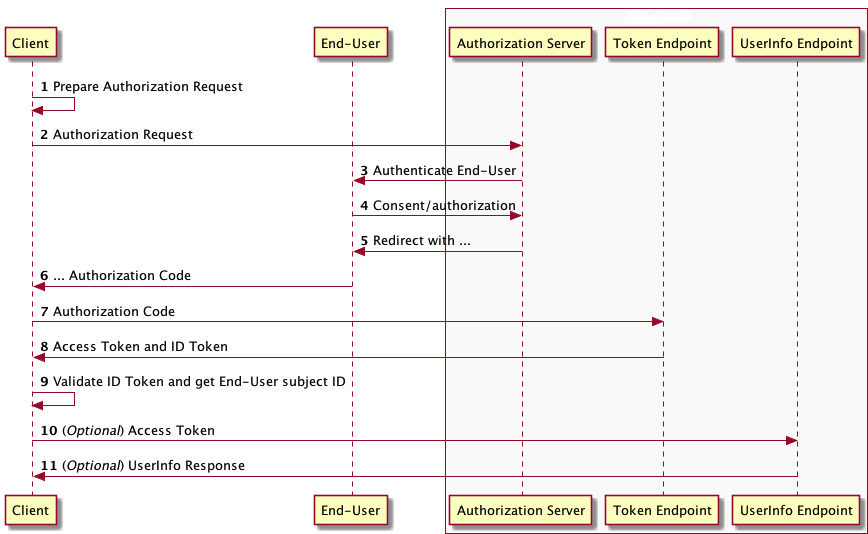
\includegraphics[width=1\textwidth]{Images/Ebert/AuthorizationCodeFlow.PNG}
	\caption{OpenID Connect Authorization Code Flow Übersicht [12]}
	\label{fig:EB_AuthorizationCodeFlow}
\end{figure} % TODO: also returns refresh token; rename authorization server to authorization endpoint?

Als erstes wird der Autorization Request vorbereitet. Diese Anfrage enthält mehrere Parameter im Query-String. Einer davon ist die Identifikationsnummer des Clients [14]. Diese ID wird bei der Registrierung des Clients beim OpenID Provider angegeben. Durch diese ID kann der OpenID Provider identifizieren, auf welche Scopes der Client Zugriff haben darf. Die Anfrage enthält auch eine Liste von gewünschten Scopes. Die später im Access Token erlaubten Scopes sind dann die Schnittmenge der gewünschten und erlaubten Scopes TODO:check if thats actually right-seems like i get auto access to some scopes. Der openid Scope muss immer in der Liste der gewünschten Scopes angegeben werden [14]. Dieser spezifiziert, dass es sich um eine OpenID Connect Anfrage handelt. Weiter muss eine 'redirect\_uri' angegeben werden. Nach erfolgreicher oder fehlgeschlagener Authentifizierung wird der Browser des Users zu dieser URI geleitet [14]. Diese URI muss beim Registrieren des Clients mit angegeben werden. Optional kann in der Anfrage eine 'state' enthalten werden. Diese kann vor Cross-Site Request Forgery (CSRF) schützen [14]. Ebenfalls optional kann eine 'nonce' angegeben werden, welche vor Replay Angriffen schützen kann [14]. 'state' und 'nonce' werden später in Kapitel TODO näher betrachtet. Listing \ref{EBAutorizationRequest} zeigt ein Beispiel für einen Autorization Request. Über den 'response\_type=code' wird der Authorization Code Flow ausgewählt. Mit 'response\_mode=fragment' wird festgelegt, dass später ein Code per URI Fragment übertragen wird. Letzteres wird später in Schritt 5 und 6 näher erläutert.

\begin{lstlisting}[caption=Beispiel Autorization Request, captionpos=b, label=EBAutorizationRequest]
GET https://keycloak/auth/realms/Test/protocol/openid-connect/auth?
	client_id=react-frontend
	&redirect_uri=https%3A%2F%2Freactfrontend.com%2F
	&state=0909ff6a-53b2-4253-8690-aff72d2cfff1
	&response_mode=fragment
	&response_type=code
	&scope=openid%20profile
	&nonce=67bad316-d8c1-45d1-9559-2a1c4726ce91
\end{lstlisting}

Im zweiten Schritt wird die Anfrage aus Schritt 1 an den Authorization Server, also den OpenID Provider, gesendet. Bei dieser Anfrage handelt es sich um eine GET HTTP-Anfrage. Das bedeutet, dass der User nach Schritt 2 nicht auf der Website des Clients, sondern auf der Website des OpenID Provider ist. Dies ist im Hinblick auf die Sicherheit wichtig, da sich der User im dritten Schritt authentisieren muss und seine Anmeldeinformationen wie z.B. Username und Passwort eingeben muss. Da dies nicht auf der Seite des Clients passiert, sind die Anmeldeinformationen des Users vom Client abgeschirmt [15]. Das bedeutet, dass der Client keine Informationen über die Anmeldeinformationen des Users hat. Der Client erhält nur die Tokens.

Das OpenID Connect Protkoll schreibt nicht vor, mit welchen Methoden der OpenID Provider den User in Schritt 3 authentifiziert [16]. Als sicherere Alternative zu Username und Passwort könnte hier z.B. auch eine Zwei-Faktor-Authentifizierung eingesetzt werden. Auch die Methode, wenn der User bereits authentifiziert ist, wird vom OpenID Connect Protokoll nicht vorgeschrieben. Zum Beispiel implementiert Keycloak das über HTTP Cookies. Nach einer erfolgreichen Authentifizierung, wird ein ID Token als KEYCLOAK\_IDENTITY Cookie für Keycloak's Authorization Endpunkt gesetzt [17]. Bei Anfragen an Keycloak's Authorization Endpunkt ist dieser Token automatisch enthalten. Der Ablauf für bereits authentifizierte User ist dann größtenteil gleich wie der für nicht authentifizierte User. Allerdings wird der User dann in Schritt 3 durch den Token, und nicht durch die Eingabe von z.B. Username und Passwort authentifiziert.

Nach erfolgreicher Authentifizierung muss der OpenID Provider in Schritt 4 sicherstellen, dass der Client zum Zugriff auf die von ihm gewünschten Scopes berechtigt ist. Im vorhinein kann der Administrator des OpenID Providers die erlaubten Scopes für jeden Client festlegen. Optional kann in diesem Schritt auch ein interaktiver Dialog mit dem User stattfinden [18]. Dabei wird dem User die Liste der gewünschten Scopes angezeigt. Der User hat hier die Möglichkeit, den Scopes zuzustimmen oder die Authentifizierung abzubrechen.

In Schritt 5 und 6 wird der User bzw. der Browser zur redirect\_uri umgeleitet. Diese URI ist im Authorization Request von Schritt 1 spezifiziert worden. Die URI enthält einen vom OpenID Provider erstellten Code im Query-String oder im URI Fragment. Dieser Code ist für den Client opak. Seine Struktur wird also nur vom OpenID Provider verstanden. Der Code enthält Informationen über die Authentifizierung der vorherigen Schritte. Dazu gehören z.B. welche Scopes im Access Token enthalten sein werden. Der Code hat eine kurze Verfallszeit [21]. Im Folgenden wird eine beispielhafte Redirect URI gezeigt.

\begin{lstlisting}[caption=Beispiel Redirect URI, captionpos=b, label=EBBeispielRedirectURI]
https://reactfrontend.com/#
	state=0909ff6a-53b2-4253-8690-aff72d2cfff1&
	code=50342949-85bb-47ba-84ab-ed890b088226.0d9f3aa9-9e37-4c
	b7-a589-06972b3cf410.ef40a086-7a64-4b49-b3f0-11dc5cf92a68
\end{lstlisting}

Durch das im Authorization Request aus Schritt 1 angegebene 'response\_mode=fragment' werden die Informationen über das URI Fragment übermittelt. Die in der Redirect URI zurückgegebene 'state' muss dieselbe sein wie in der Autorization Request [20]. Das verhindert CSRF, was später in Sektion TODO näher erläutert wird.

% state csrf explained https://stackoverflow.com/questions/58823560/what-kind-of-csrf-attack-does-state-parameter-prevent-in-oauth2-based-authentica > entweder hier oder später

Der Code kann am Token Endpoint des OpenID Connect Providers zu einem ID, Access, und optional einem Refresh Token ausgetauscht werden [19]. Dies wird in Schritt 7 und 8 per HTTP POST Anfrage durchgeführt [20]. Um potenzielle Replay Angriffe zu verhindern, kann dieser Code nur einmal verwendet werden [21].

Durch die POST Anfrage werden die Tokens im HTTP Response Body zurückgegeben. Dadurch werden sie nicht dem Browser ausgesetzt [22] und z.B. nicht im Browserverlauf gespeichert [23]. Im Gegensatz dazu wurden Informationen wie z.B. der Code dem Browser ausgesetzt. Da der Access Token eine längere Verfallszeit hat und potentiell nicht widerrufen werden kann, sollte der Browser diesen aus Sicherheitsgründen nicht speichern [23].

In Schritt 8 muss der ID Token validiert werden. Dazu gehört zum Beispiel das Überprüfen der Signatur des Tokens [24]. Wird im Authorization Request in Schritt 1 eine nonce angegeben, dann muss der ID Token einen nonce Claim enthalten [24]. Die nonce des Authorization Request muss mit der nonce des ID Tokens übereinstimmen [24]. Außerdem muss die ID des Clients im 'aud' Claim des ID Tokens enthalten sein, die 'iss' muss die ID des OpenID Providers enthalten, und der ID Token darf nicht bereits abgelaufen sein [24]. Der 'aud' und 'iss' Claim wurden in Sektion \ref{EB_End-User} erläutert. Optional können weitere Validierungen stattfinden. Zum Beispiel kann ein Token abgelehnt werden, wenn die auth\_time zu weit in der Vergangenheit liegt [24]. Der interessierte Leser findet unter [24] alle weiteren optionalen Validierungen.

Wie bereits in Sektion \ref{EB_AccessToken} erläutert kann der ID Token nicht alle User Claims enthalten. Die durch den scope Claim des Access Token zugelassenen User Claims können abschließend optional über den UserInfo Endpunkt angefordert werden.

Als Alternative zum Authorization Code Flow bietet das OpenID Connect Protokoll den Implicit Flow und den Hybrid Flow an, um einen User zu authentifizieren. Diese zwei Alternativen haben beide eine bessere Performance [26] und eine kürzere Latenz als der Authorization Code Flow [25]. Trotzdem sollten beide, zumindest mit Keycloak, aus Sicherheitsgründen nicht verwendet werden, da bei beiden Access Tokens über den Browserverlauf geleakt werden können [26] [23].

% kurz erwähnen dass sich clients dynamisch oder alternativ dass admin das macht in openid provider? kurz?

\subsubsection{Zugriff auf geschützte Ressourcen} \label{EB_Zugriff auf geschützte Ressourcen}

Der in dieser Sektion vorgestellte Prozess ermöglicht den Zugriff auf Ressourcen in anderen Clients, welche für die authentifizierten und autorisierten User beschränkt ist. Diese anderen Clients werden dabei auch Ressourcen Server genannt. Dabei wird der Access Token dem Ressourcen Server präsentiert. Der Standard schreibt nicht vor, wie dieses Präsentieren des Access Tokens stattfinden soll [28]. Allerdings gibt der Standard an, dass der Access Token üblicherweise über den Authorization Header der HTTP Anfrage als sogenannten Bearer Token übermittelt wird [28]. 

Bearer Token bedeutet, dass jeder, der im Besitz des Tokens ist, den Token wie jeder andere einsetzten kann [29]. Das bedeutet, dass der Ressourcen Server den Token an andere Clients senden kann, um von diesen Ressourcen abzurufen. Das kann z.B. in einer Microservice Architektur vorkommen [31]. Aus diesem Grund sollte man aus Sicherheitsgründen, vor allem wenn es möglicherweise nicht vertrauenswürdige Clients gibt, die erlaubten Scopes im Access Tokens analysieren und diese so weit wie möglich beschränken. Außerdem kann, wie in Sektion \ref{EB_AccessToken} beschrieben ist, über den Audience Claim im Access Token angegeben werden, für welche Clients der Access Token bestimmt ist. Der Ressourcen Server sollte validieren, dass seine Client ID im Audience Claim enthalten ist, bevor er angeforderte geschützte Daten zurücksendet [30].

\subsubsection{Validieren des Access Token}

Außer der im letzten Abschnitt erläuterten Validierung des Audience Claims müssen weitere Informationen überprüft werden, bevor geschützte Daten vom Ressourcen Server herausgegeben werden. Dazu gehört die Überprüfung, ob der Token bereits abgelaufen ist. Außerdem kann ein Ressourcen Server, basierend auf den erlaubten Scopes des Access Tokens, Entscheidungen treffen. Zum Beispiel kann er die Herausgabe geschützter Daten aufgrund nicht vorhandener erlaubten Scopes verweigern.

Zusätzlich muss der Access Token validiert werden. Grundsätzlich gibt es zwei Verschiedene Varianten, wie der Access Token validiert werden kann. In dieser Sektion werden diese als Online und als Offline Variante bezeichnet.

\begin{figure}[!h]
	\centering
	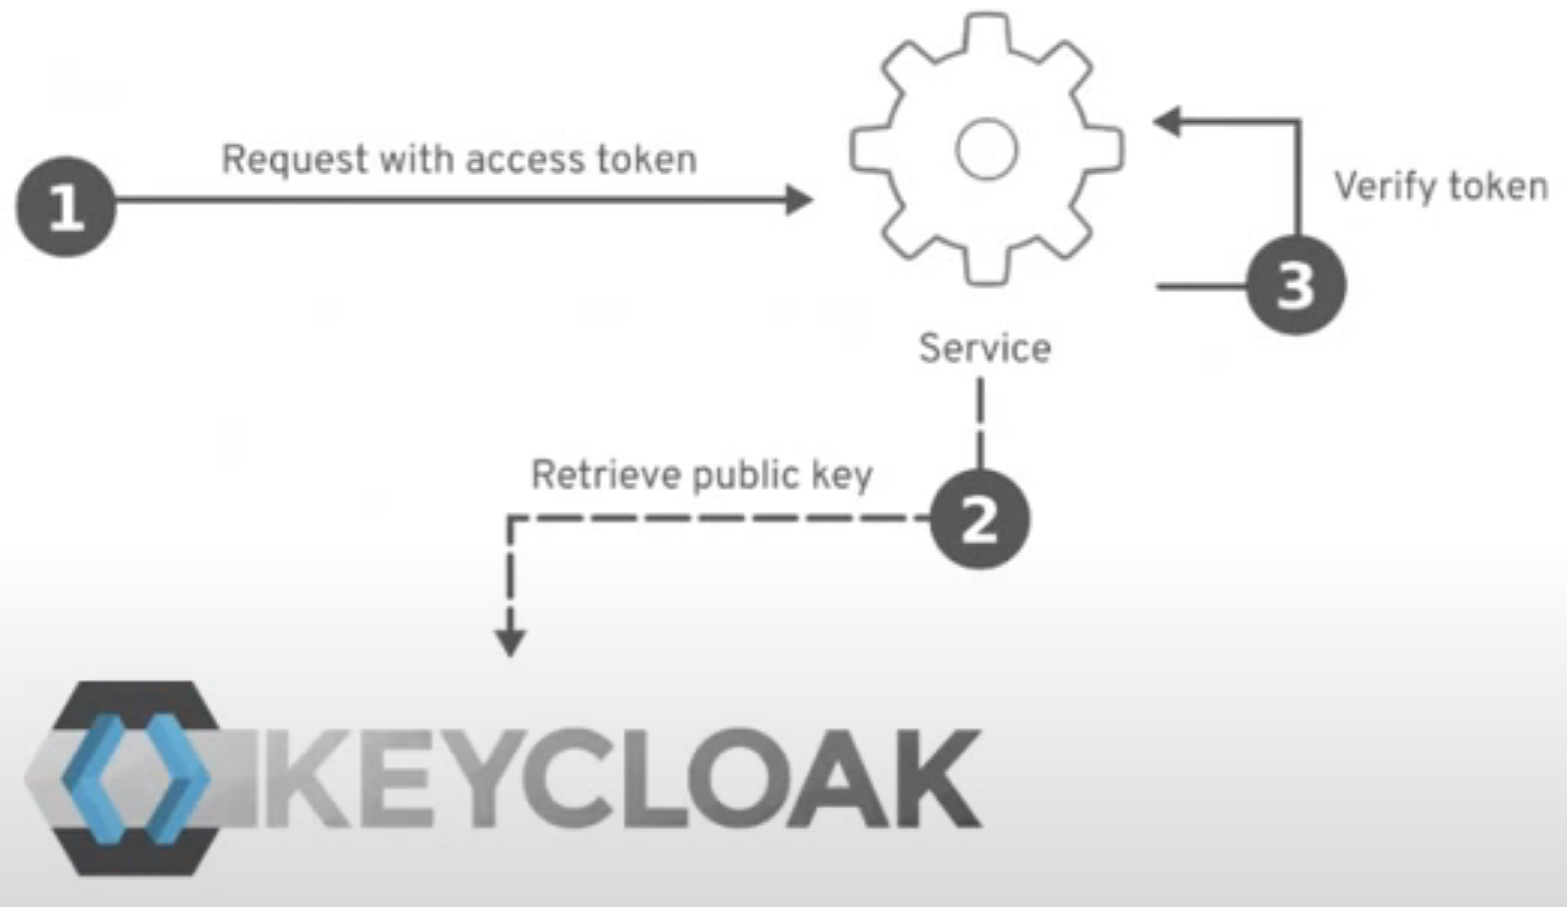
\includegraphics[width=.8\textwidth]{Images/Ebert/VerifyAccessTokenOffline.PNG}
	\caption{Access Token Verifizierung Offline Variante [32]}
	\label{fig:EB_Access Token Verifizierung Offline Variante}
\end{figure}

In Abbildung \ref{fig:EB_Access Token Verifizierung Offline Variante} ist eine Übersicht der Offline Variante gezeigt. Dabei wird der Öffentliche Schlüssel, dessen Privater Schlüssel vom OpenID Provider für die Signatur des Access Token verwendet wurde, vom OpenID Provider abgerufen. In der Abbildung ist Keycloak der OpenID Provider und der Client wird als Service bezeichnet. Der Client kann die Signatur des Access Token mit dem Öffentliche Schlüssel validieren.

Bei der Offline Variante wird der Public Key oft gecached [32]. Das Verringert die Latenz der Anfrage und die Auslastung des OpenID Provider Servers [32]. Allerdings kann der Access Token dann nicht widerrufen und invalidiert werden. Aus diesem Grund haben Access Tokens im OpenID Connect Protokoll eine kurze Verfallszeit. Trotzdem bleibt dabei ein Zeitraum, in dem der erlaubte Zugriff eines Users durch seine bereits existierenden Access Tokens nicht eingeschränkt werden kann. Um dieses Problem zu lösen, kann die Online Variante zur Validierung verwendet werden. % theorietisch könnte client bescheid gegeben werden

\begin{figure}[!h]
	\centering
	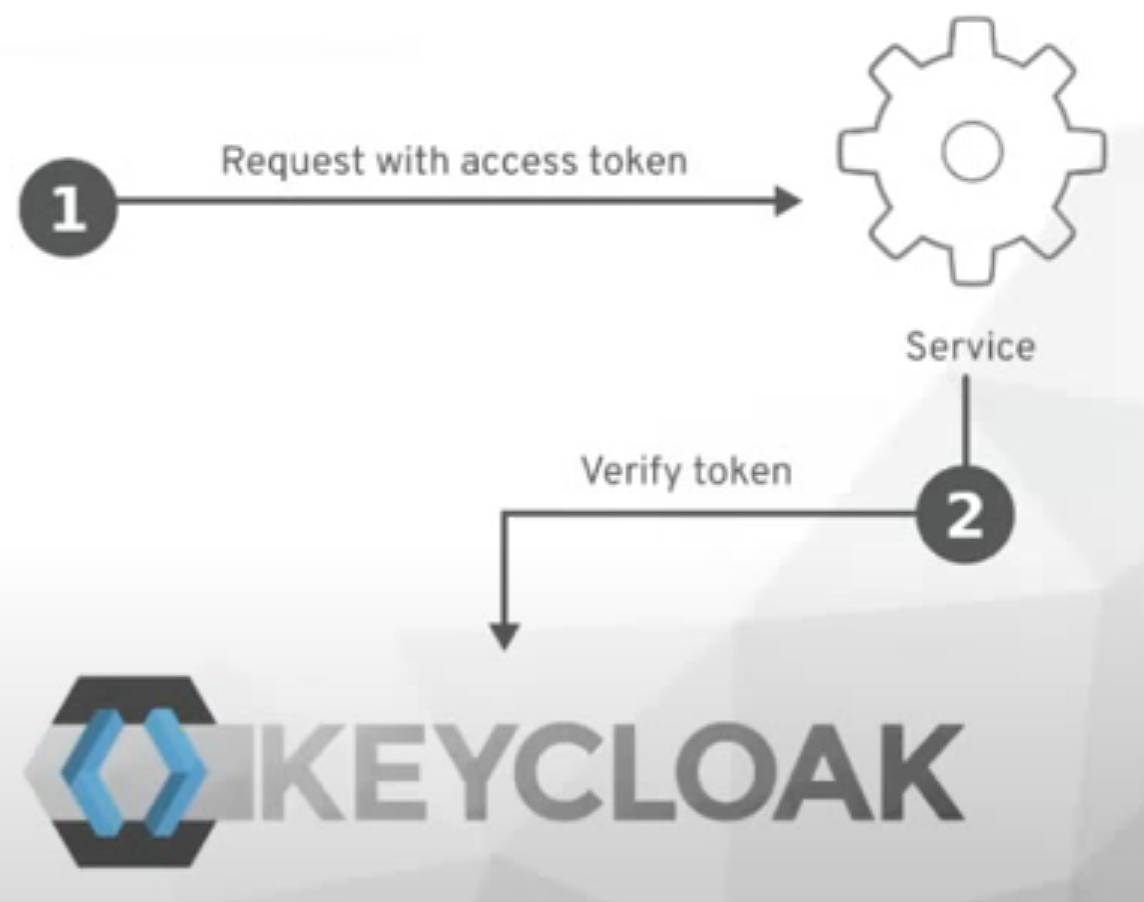
\includegraphics[width=.6\textwidth]{Images/Ebert/VerifyAccessTokenOnline.PNG}
	\caption{Access Token Verifizierung Online Variante [32]}
	\label{fig:EB_Access Token Verifizierung Online Variante}
\end{figure}

Eine Übersicht der Online Variante wird in Abbildung \ref{fig:EB_Access Token Verifizierung Online Variante} gezeigt. Hier wird der Access Token bei jeder Anfrage an den OpenID Provider gesendet, um ihn dort zu verifizieren. Der OpenID Provider kann dann zusätzlich überprüfen, ob sich der User ausgeloggt hat, ob der User gesperrt wurde, oder ob ein Administrator des OpenID Providers alle Access Tokens bis zu einem bestimmen Zeitpunkt gesperrt hat [32]. Diese Maßnahmen greifen dann mit sofortiger Wirkung. Der Nachteil der Online Variante ist, dass jede Anfrage eine höhere Latenz hat, und dass der OpenID Provider Server eine höhere Auslastung hat. Keycloak bietet für diese Variante einen Endpunkt zur Validierung an. 

Den Nachteilen der Online Variante kann entgegengewirkt werden. Wie bereits in Sektion \ref{EB_Einleitung} erwähnt, bietet Keycloak die Möglichkeit an, mehrere Keycloak Instanzen zu verwenden [33]. Dadurch kann die Last für den OpenID Provider auf mehrere Server verteilt werden. Darüber hinaus kann die Latenzzeit reduziert werden, indem z.B. der OpenID Provider Server und der Ressourcen Server im selben Rechenzentrum oder Rack betrieben werden.

% increases the day of responses and increases the processing needed

% check if needed scope. can depending on scope and validate signature; check if in aud claim. isnt there list of all checks??

% https://tools.ietf.org/html/rfc6749#section-7

% Der Access Token wird für die Authorisierung des Users verwendet. Man kann ihn als Schlüssel für Ressourcen interpretieren. Er enthält Informationen, auf welche Ressourcen und Clients man mit dem Access Token Zugriff hat. In Web-SSO kann der Access Token z.B. als Bearer Token im HTTP Authentication Header an Backend Services enthalten sein. 

\section{Threat Model}

% https://en.wikipedia.org/wiki/Threat_model > essentially What can go wrong? and What can we do about it?
% https://www.keycloak.org/docs/latest/server_admin/index.html#threat-model-mitigation > seems good 


% [1] https://openid.net/specs/openid-connect-core-1_0.html
% [2] https://tools.ietf.org/html/rfc6749#section-1.1
% [3] https://www.keycloak.org/docs/latest/server_admin/index.html#_clients
% [4] https://openid.net/specs/openid-connect-core-1_0.html#UserInfo
% [5] https://tools.ietf.org/html/rfc7515
% [6] https://www.keycloak.org/docs/latest/server_admin/#social-identity-providers
% [7] https://identityserver.github.io/Documentation/docsv2/overview/terminology.html#:~:text=A%20client%20is%20a%20piece,a%20relying%20party%20or%20RP).&text=Examples%20for%20clients%20are%20web,%2C%20SPAs%2C%20server%20processes%20etc.
% [8] https://auth0.com/docs/tokens#id-tokens
% [9] https://identityserver.github.io/Documentation/docsv2/overview/terminology.html
% [10] https://auth0.com/docs/tokens#access-tokens
% [11] https://openid.net/specs/openid-connect-core-1_0.html#ScopeClaims
% [12] https://medium.com/@aminsaqi/a-survey-on-sso-authentication-protocols-security-and-performance-287dcb634bdd
% [13] https://tools.ietf.org/html/rfc6749
% [14] https://openid.net/specs/openid-connect-core-1_0.html#AuthRequest
% [15] https://www.keycloak.org/docs/latest/server_admin/#how-does-security-work
% [16] https://openid.net/specs/openid-connect-core-1_0.html#Authenticates
% [17] https://blog.codecentric.de/2016/08/single-sign-mit-keycloak-als-openid-connect-provider/
% [18] https://openid.net/specs/openid-connect-core-1_0.html#Consent
% [19] https://openid.net/specs/openid-connect-core-1_0.html#TokenEndpoint
% [20] https://openid.net/specs/openid-connect-basic-1_0.html#CodeOK
% [21] https://www.keycloak.org/docs/latest/server_admin/index.html#authorization-code-flow
% [22] https://connect2id.com/learn/openid-connect
% [23] https://www.keycloak.org/docs/latest/server_admin/index.html#implicit-flow
% [24] https://openid.net/specs/openid-connect-core-1_0.html#IDTokenValidation
% [25] https://openid.net/specs/openid-connect-basic-1_0.html#CodeFlow
% [26] https://www.keycloak.org/docs/latest/securing_apps/#_javascript_implicit_flow
% [27] https://tools.ietf.org/html/rfc6750
% [28] https://tools.ietf.org/html/rfc6749#section-7
% [29] https://tools.ietf.org/html/rfc6750#section-1.2
% [30] https://www.keycloak.org/docs/latest/server_admin/#_audience
% [31] https://youtu.be/mdZauKsMDiI?list=WL&t=745
% [32] https://youtu.be/mdZauKsMDiI?list=WL&t=630
% [33] https://www.keycloak.org/docs/latest/server_installation/#_standalone-ha-mode
% [34] https://www.researchgate.net/publication/309225903_A_Review_on_Single_Sign_on_Enabling_Technologies_and_Protocols
% [35] https://www.keycloak.org/docs/latest/securing_apps/#openid-connect-3
% [36] https://www.npmjs.com/package/@react-keycloak/web
% [37] https://www.keycloak.org/docs/latest/server_admin/index.html#openid-connect-vs-saml
% [38] https://www.researchgate.net/publication/257743941_A_Survey_on_Single_Sign-On_Techniques
% [39]











